% ====================================================================
% VİZE RAPOR ŞABLONU – Türk Masalları Derlemesi Web Sayfası
% --------------------------------------------------------------------
% DERLEME: Overleaf'te Menu > Compiler > XeLaTeX (pdfLaTeX de çalışır).
%
% KURALLAR (şablonu kullanmadan önce okuyun):
%  1. Bölüm başlıklarını SİLMEYİN ve sırasını DEĞİŞTİRMEYİN.
%  2. [KÖŞELİ PARANTEZ] içindeki ve gri renkli açıklama metinlerini
%     kendi bilgilerinizle değiştirin; açıklama metinlerini silin.
%  3. MEBİS'e YALNIZCA bu raporun PDF'ini yükleyin.
%     ZIP ve HTML dosyası YÜKLEMEYİN. Tüm kontroller GitHub'dan yapılır.
%  4. Kapaktaki GitHub ve YouTube bağlantıları doğru ve tıklanabilir
%     olmalıdır. Teslimden önce PDF'teki bağlantılara tıklayıp deneyin.
%  5. Haftalık katkı tablosundaki görseller için resim dosyalarını
%     (hafta1.png, hafta2.png, ...) Overleaf projesine yükleyin.
%     Dosya adlarında boşluk ve Türkçe karakter kullanmayın.
%     Resim yoksa tabloda "görsel ekleyin" kutusu görünür.
%  6. Yapay zekâ kullandıysanız Bölüm 5'i doldurun.
% ====================================================================
\documentclass[12pt,a4paper]{article}

\usepackage{iftex}
\ifPDFTeX
  \usepackage[T1]{fontenc}
  \usepackage[utf8]{inputenc}
\else
  \usepackage{fontspec}
\fi
\usepackage[turkish]{babel}
\usepackage[margin=2.4cm]{geometry}
\usepackage{setspace}
\usepackage{graphicx}
\usepackage{booktabs}
\usepackage{longtable}
\usepackage{array}
\usepackage{colortbl}
\usepackage{xcolor}
\usepackage{enumitem}
\usepackage{listings}
\usepackage{amssymb}
\usepackage{caption}
\usepackage{fancyhdr}
\usepackage{hyperref}

\onehalfspacing
\setlength{\parindent}{0pt}
\setlength{\parskip}{6pt}
\setlist{itemsep=2pt, topsep=4pt}
\hypersetup{colorlinks=true, linkcolor=blue!50!black, urlcolor=blue!50!black}

\definecolor{ana}{HTML}{14325C}
\definecolor{acik}{HTML}{EEF2F8}

\lstset{basicstyle=\ttfamily\small, backgroundcolor=\color{acik},
  frame=single, rulecolor=\color{ana}, breaklines=true,
  columns=fullflexible, keepspaces=true, showstringspaces=false}

\pagestyle{fancy}
\fancyhf{}
\fancyhead[L]{Türk Masalları}
\fancyhead[R]{Vize Raporu}
\fancyfoot[C]{\thepage}

% ---------- Yardımcı komutlar ----------
% Gri açıklama metni (silinecek yönergeler için)
\newcommand{\aciklama}[1]{{\color{gray}\itshape (#1)}}

% Haftalık tablo görseli: dosya yoksa "görsel ekleyin" kutusu çıkar
\newcommand{\haftagorsel}[1]{%
  \IfFileExists{#1}{%
    \includegraphics[width=\linewidth,height=4.2cm,keepaspectratio]{#1}%
  }{%
    \fbox{\parbox[c][2.6cm][c]{\dimexpr\linewidth-2\fboxsep-2\fboxrule\relax}{%
      \centering\small\color{gray} Ekran görüntüsü / görsel ekleyin\\ \texttt{#1}}}%
  }%
}
% Haftalık katılım kutuları (işaretlemek için $\square$ yerine $\boxtimes$ yazın)
\newcommand{\katilimkutulari}{\par\vspace{3pt}\small $\square$ Ders içinde katılım sergiledim\par $\square$ Telafi yaptım}

% Ek görsel: dosya yoksa hiçbir şey göstermez
\newcommand{\haftaek}[1]{%
  \IfFileExists{#1}{\\[4pt]\includegraphics[width=\linewidth,height=4.2cm,keepaspectratio]{#1}}{}%
}

% ---------- Kapak bilgileri ----------
\newcommand{\universite}{İstanbul Medipol Üniversitesi / Görsel İletişim Tasarımı Bölümü}
\newcommand{\dersadi}{Programlamaya Giriş}
\newcommand{\hocaadi}{Meral Şentürk}
\newcommand{\ogrenciadi}{Zeynep Sıla Kuştu}
\newcommand{\ogrencino}{86260034}
\newcommand{\projeadi}{Türk Masalları}
% Bağlantıları tam adres olarak yazın (https:// ile başlayarak)
\newcommand{\githublink}{\url{https://github.com/zeynepsilakst-web/turk-masallari}}
\newcommand{\youtubelink}{\url{https://youtu.be/jac8dAwPfN8}}

\begin{document}

% ====================================================================
% KAPAK
% ====================================================================
\begin{titlepage}
\centering
\vspace*{1cm}
{\large \universite \par}
\vspace{1.8cm}
{\Huge\bfseries\color{ana} \projeadi \par}
\vspace{0.4cm}
{\Large Türk Masalları Derlemesi Web Sayfası \par}
{\large Vize Raporu \par}
\vspace{1.8cm}
{\large \textbf{Ders:} \dersadi \par}
{\large \textbf{Öğretim Üyesi:} \hocaadi \par}
\vspace{1.2cm}
{\large \textbf{Hazırlayan:} \ogrenciadi \par}
{\large \textbf{Öğrenci No:} \ogrencino \par}
\vspace{1.8cm}
\fbox{\parbox{0.88\linewidth}{\centering\vspace{6pt}
{\large\bfseries Proje Bağlantıları}\\[8pt]
\textbf{GitHub deposu:}\\ \githublink \\[8pt]
\textbf{YouTube sunum videosu:}\\ \youtubelink
\vspace{6pt}}}
\vfill
{\large \today \par}
\end{titlepage}

\tableofcontents
\newpage

% ====================================================================
\section{Giriş}
% ====================================================================

\subsection{Proje Özeti}
Bu projede Türk halk anlatı geleneğinden seçtiğim on masalı bir araya getiren bir web sayfası hazırladım. Amacım, masalları okumaya uygun, sade ve konuya yakışan bir arayüzle sunmaktı. Sayfa tek bir HTML dosyasından oluşuyor; tasarım için içsel CSS, sayfanın işlevleri için içsel JavaScript kullandım. Ziyaretçi masal listesinden bir masala tıklayınca masal bir pencerede açılıyor; arama kutusuyla masalları adına göre süzebiliyor ve okurken yazı boyutunu değiştirebiliyor. Sayfa harici bir dosya ya da kütüphane kullanmadığı için internet bağlantısı olmadan çalışıyor; yalnızca görseller yanındaki \texttt{gorseller} klasöründe duruyor. Bu raporda masal seçimimi, tasarım kararlarımı, kodun nasıl çalıştığını, yapay zekâ kullanımımı ve haftalık çalışmalarımı anlatıyorum.

\subsection{Gereksinimlerin Karşılanması}
\begin{center}
\rowcolors{2}{acik}{white}
\begin{tabular}{@{}p{8.2cm}c@{}}
\toprule
\rowcolor{ana}\textcolor{white}{\textbf{Gereksinim}} & \textcolor{white}{\textbf{Durum}} \\
\midrule
Masal sayısı 8--12 arasında (10 masal)         & $\boxtimes$ \\
Tek HTML dosyası                                    & $\boxtimes$ \\
Stil kodları içsel (\texttt{<style>} içinde)        & $\boxtimes$ \\
Betik kodları içsel (\texttt{<script>} içinde)      & $\boxtimes$ \\
İnternetsiz açılıp çalışıyor                        & $\boxtimes$ \\
JavaScript sayfada anlamlı bir işlev görüyor        & $\boxtimes$ \\
Masal metinleri kendi cümlelerimle yazıldı          & $\boxtimes$ \\
Sayfa telefonda da düzgün görünüyor                 & $\boxtimes$ \\
\bottomrule
\end{tabular}
\end{center}

% ====================================================================
\section{Masalların Seçimi}
% ====================================================================
Masalların hepsini T.C. Kültür ve Turizm Bakanlığının Kültür Portalı'ndan seçtim. Bu masalları seçmemin nedeni, Türk kültürünün sözlü anlatı geleneğini farklı konular ve karakterler üzerinden tanımak ve tanıtmaktır. Derlemede; iyilik, sabır, sevgi, cesaret, kıskançlık, dostluk ve kurnazlık gibi temaları işleyen anlatılara yer verdim. Kimi masallarda olağanüstü varlıklar ve sihirli nesneler öne çıkarken kimilerinde gündelik yaşamdan izler, mizah ve halkın yaşam tecrübesi görülür. Farklı yörelerden ve derleyicilerden gelen bu anlatıların bir arada bulunmasının, masalların dilimizi, hayal gücümüzü ve kültürel hafızamızı nasıl taşıdığını göstermesini istedim. Bu nedenle seçtiğim masalları, olay örgülerini ve sonlarını koruyarak daha anlaşılır, akıcı ve günümüz Türkçesine yakın bir dille yeniden düzenledim.

\begin{longtable}{@{}cp{4cm}p{3cm}p{5.4cm}@{}}
\toprule
\textbf{No} & \textbf{Masal} & \textbf{Tür} & \textbf{Seçilme nedeni} \\
\midrule
\endhead
1 & Peri Kızı & Olağanüstü masal & Göl dibindeki peri kızları ve konuşan küpler gibi masalsı unsurları ilgimi çekti. \\
2 & Çobanla Köpeği & Olağanüstü masal & İyiliğin karşılık bulmasını, yardım edilen hayvanların sonunda kahramanı kurtarmasıyla anlatıyor. \\
3 & İnatçı Horoz & Zincirleme masal & Kısa ve eğlenceli; olayların zincir gibi birbirine bağlanmasıyla derlemeye farklı bir tür kattı. \\
4 & Keloğlan ve Altın Bülbül & Olağanüstü masal & Türk masallarının en bilinen kahramanı Keloğlan'ın yer aldığı bir masal olsun istedim. \\
5 & Kurnaz Kurt & Hayvan masalı & Derlemeye bir hayvan masalı eklemek istedim; kurdun kurnazlığı masala mizah katıyor. \\
6 & Reyhan Güzeli ile Padişah Oğlu & Gerçekçi masal & Olağanüstü varlıklar yerine zekâsıyla öne çıkan bir kız kahramanı anlatıyor. \\
7 & Tuz Kadar Sevgi & Olağanüstü masal & Sevginin değerinin tuz örneğiyle anlatılması ilgimi çekti. \\
8 & Üç Turunçlar & Olağanüstü masal & Turunçtan çıkan kızlar ve dönüşümleriyle en masalsı hikâyelerden biri. \\
9 & Kırk Dost & Gerçekçi masal & Para varken dost olan, para gidince sırt çeviren insanları anlatan ders veren bir masal. \\
10 & İncili Çadır & Olağanüstü masal & Yeraltı sarayı ve incili çadır gibi etkileyici sahneleri olan bir aşk masalı. \\
\bottomrule
\end{longtable}

% ====================================================================
\section{Tasarım Kararları}
% ====================================================================

\subsection{Konuya Uygunluk}
Sayfanın renklerini geleneksel Türk sanatlarından aldım: Kırmızıyı kilimlerdeki kök boyadan, maviyi İznik çinilerinden, altın sarısını minyatürlerden esinlenerek seçtim. Krem rengi zemin, eski bir kitap sayfasını hatırlatıyor ve masal okuma duygusunu destekliyor. Masalların ilk harfini eski el yazması kitaplardaki gibi büyük ve kırmızı yaptım; masal görsellerini de minyatür kitaplarındaki resimleri andıran çift çizgili altın bir çerçeveye aldım. Ana sayfanın üstündeki lale ve rumi motifli kenarlık ile masal penceresinin köşe motifleri İznik çinisi ve tezhip süslemelerinden esinleniyor. Bütün masal görsellerini aynı minyatür üslubunda ürettim; böylece sayfa baştan sona tek bir görsel dil konuşuyor.

\subsection{Renk Paleti ve Yazı Tipi}
\begin{center}
\rowcolors{2}{acik}{white}
\begin{tabular}{@{}llp{6.4cm}@{}}
\toprule
\rowcolor{ana}\textcolor{white}{\textbf{Ad}} & \textcolor{white}{\textbf{Kod}} & \textcolor{white}{\textbf{Nerede / neden kullandınız?}} \\
\midrule
\relax Kök boya kırmızısı & \texttt{\#8E2B23} & Başlıklar, büyük ilk harf, pencerenin üst çizgisi; kilimlerdeki kök boyayı hatırlatıyor. \\
\relax Çini mavisi & \texttt{\#1D4E6B} & Masal butonlarının sol şeridi, arama kutusu ve alt yazılar; İznik çinilerinden. \\
\relax Altın sarısı & \texttt{\#C49A3A} & Görsellerin çift çizgili çerçevesi ve vurgular; minyatürlerdeki altın yaldızı hatırlatıyor. \\
\relax Georgia & -- & Başlık ve metinde aynı tırnaklı yazı tipi; kitap havası veriyor, okunaklı ve her bilgisayarda bulunduğu için internetsiz çalışıyor. \\
\bottomrule
\end{tabular}
\end{center}

\subsection{Okunabilirlik, Gezinme ve Duyarlı Tasarım}
\begin{itemize}
  \item \textbf{Okunabilirlik:} Masal metni 18 piksel boyutunda ve satır aralığı geniş. Satır uzunluğunu yaklaşık 65 harfle sınırladım, çünkü çok uzun satırları okumak yorucu oluyor. Koyu kahve metin rengi krem zemin üzerinde güçlü bir karşıtlık oluşturuyor. Okuyucu masal penceresindeki A$-$ ve A+ düğmeleriyle yazı boyutunu kendine göre ayarlayabiliyor.
  \item \textbf{Gezinme:} Bütün masallar ana sayfada numaralı bir liste hâlinde duruyor; tek tıklamayla açılıyor. Arama kutusuna masalın adından birkaç harf yazmak listeyi hemen süzüyor. Masal penceresi $\times$ düğmesiyle, pencerenin dışına tıklayarak ya da Esc tuşuyla kapanıyor.
  \item \textbf{Duyarlı tasarım:} Telefonda kenar boşlukları daralıyor, başlık ve yazılar ekrana göre küçülüyor, görseller ve kenarlık ekrandan taşmıyor. Masal penceresi telefonda neredeyse bütün ekranı kaplıyor.
  \item \textbf{Tutarlılık:} Renkleri CSS değişkenleriyle tek bir yerde tanımladım ve bütün sayfada yalnızca bu renkleri kullandım. Başlıklarda hep aynı kırmızıyı, butonlarda ve pencerelerde aynı kenarlık ve boşluk düzenini kullandım. Kaynakça penceresi de masal penceresiyle aynı görünümde.
\end{itemize}

\subsection{Ekran Görüntüleri}
\begin{figure}[h]
  \centering
  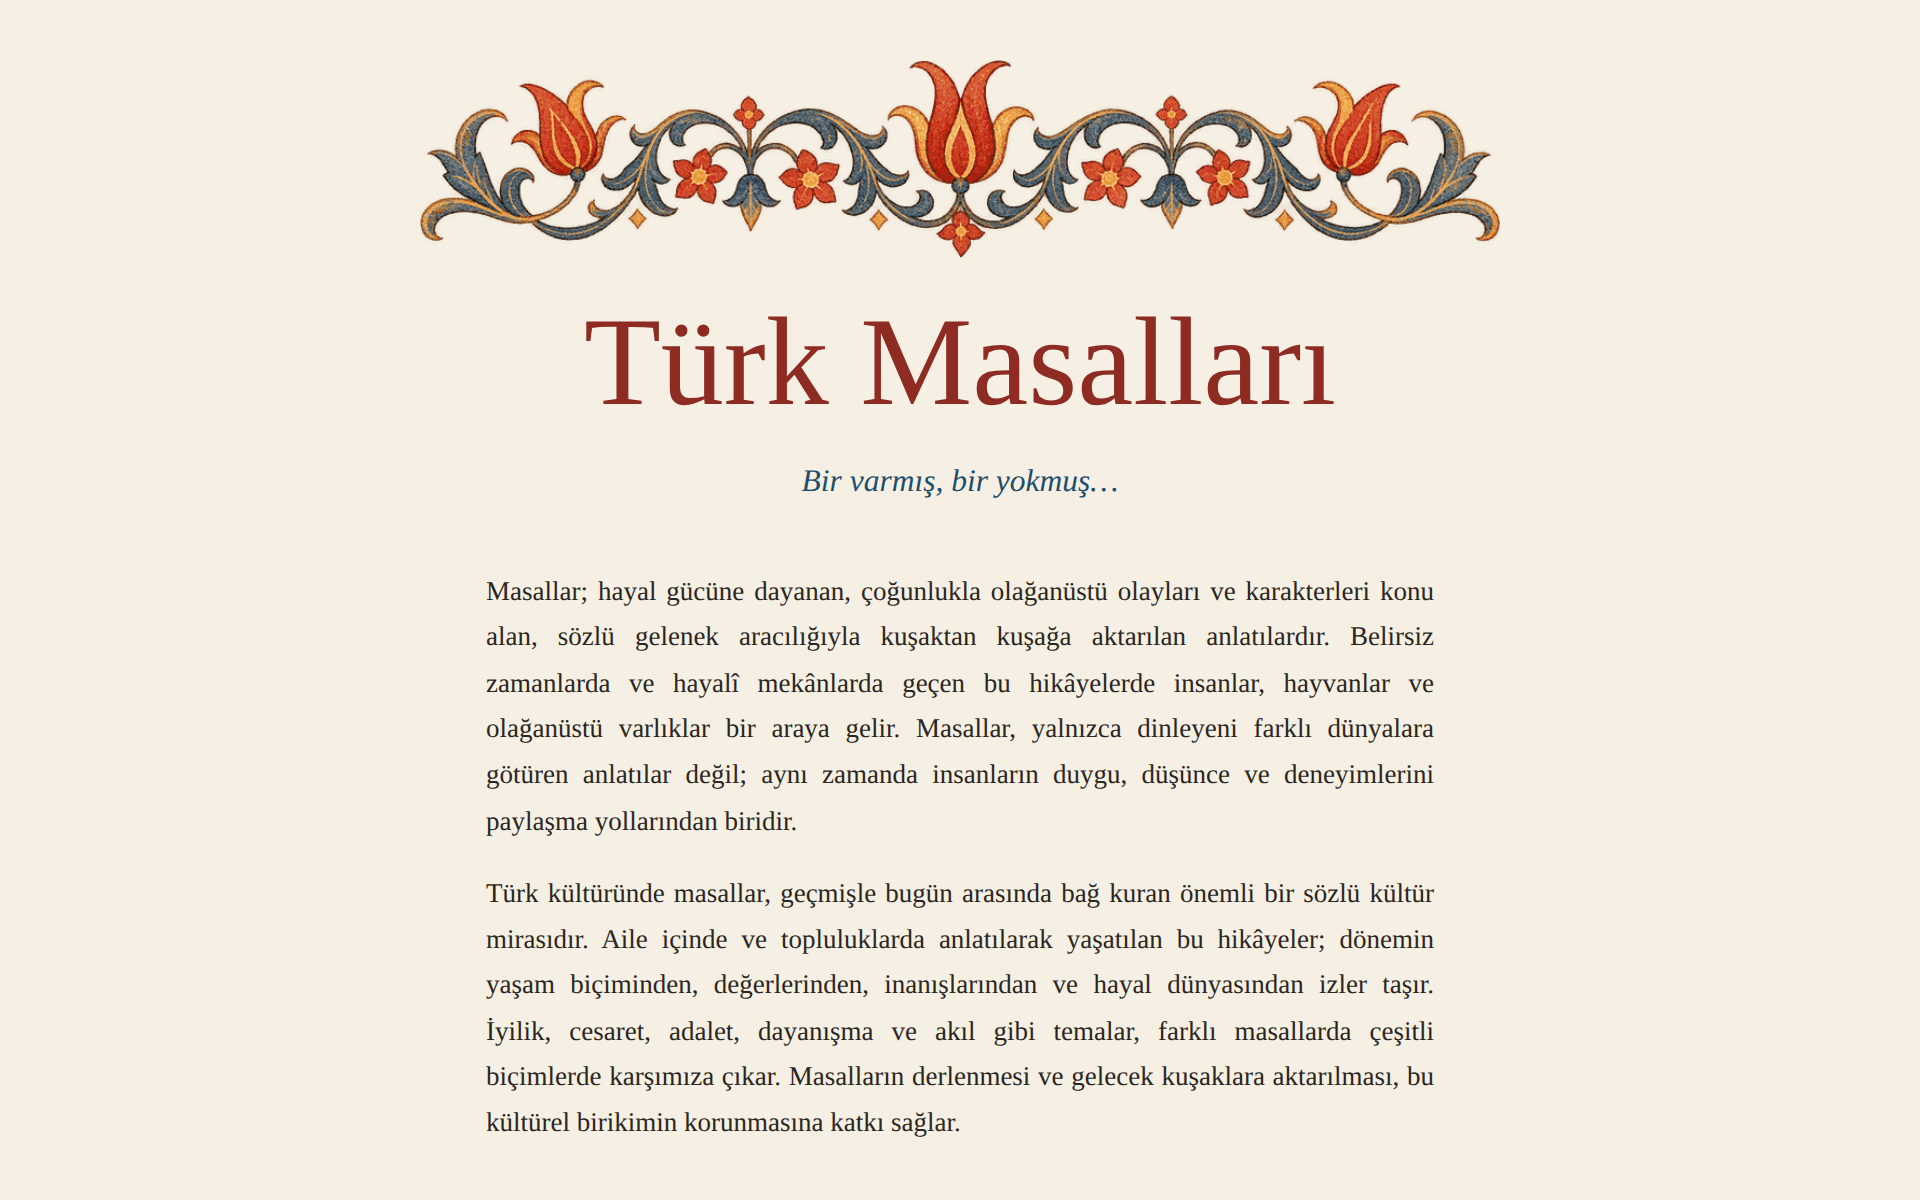
\includegraphics[width=0.9\textwidth]{ekran-masaustu.png}
  \caption{Sayfanın bilgisayar görünümü}
\end{figure}
\begin{figure}[h]
  \centering
  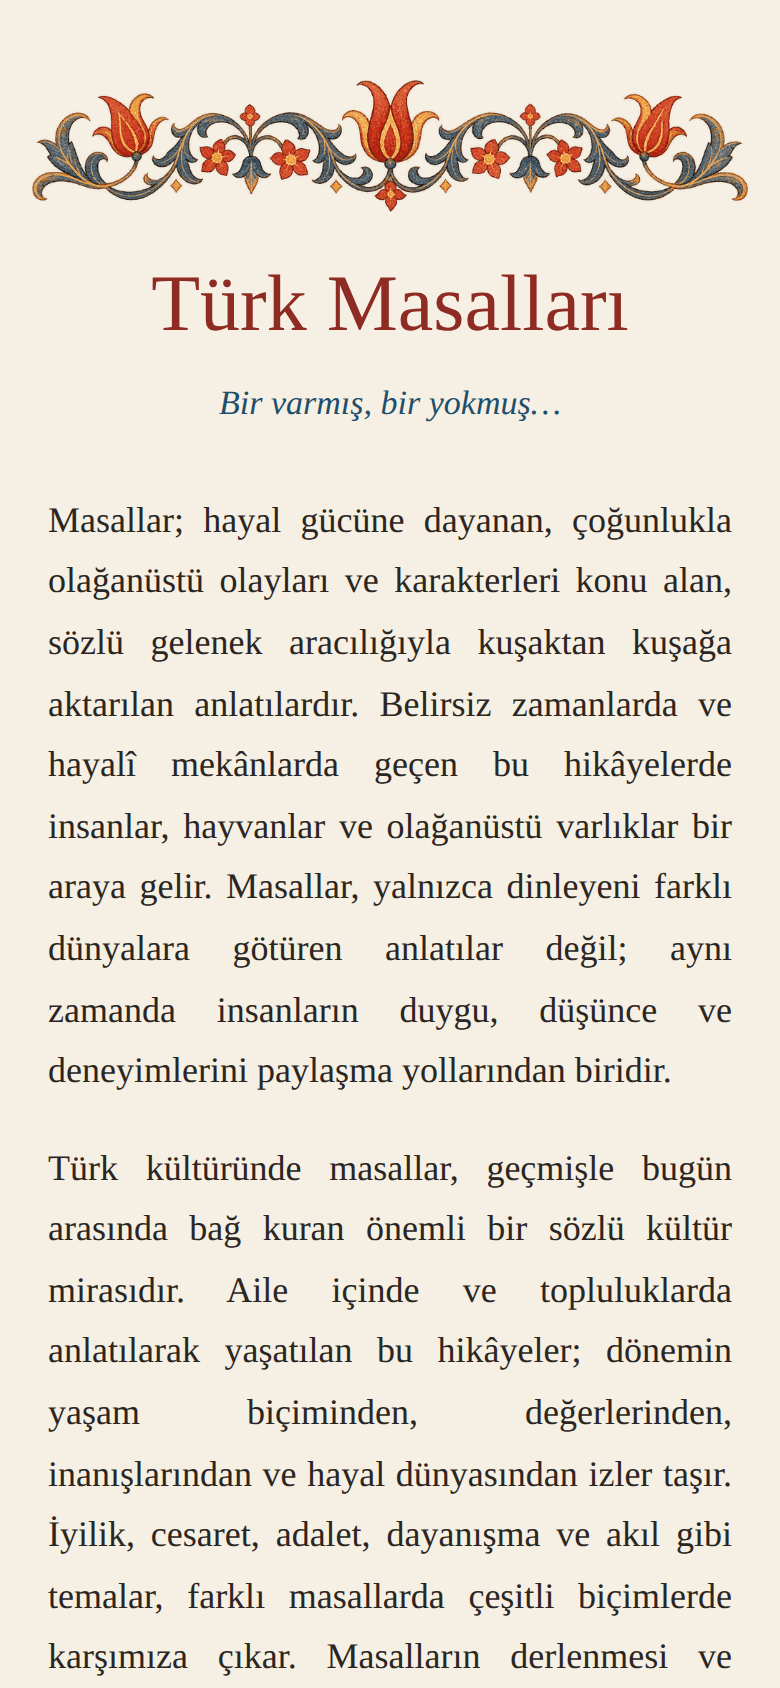
\includegraphics[width=0.35\textwidth]{ekran-mobil.png}
  \caption{Sayfanın telefon görünümü}
\end{figure}

% ====================================================================
\section{Gerçekleştirme}
% ====================================================================

\subsection{HTML Yapısı}
Sayfa yukarıdan aşağıya şu bölümlerden oluşuyor: kenarlık görseli ve başlığın bulunduğu \texttt{<header>}, masallar hakkında kısa bir tanıtım yazısı, arama kutusu ve masal listesinin bulunduğu \texttt{<main>}, hazırlayan bilgisi ve kaynakça butonunun bulunduğu \texttt{<footer>}. Her masal bir \texttt{<button>} etiketi; butonlara \texttt{data-masal} niteliğiyle 0'dan başlayan bir sıra numarası verdim. Masalın açıldığı pencereyi ve kaynakça penceresini \texttt{<dialog>} etiketiyle yaptım. Arama kutusu bir \texttt{<input>}, görseller \texttt{<img>} etiketi. Sayfada bir tane olan öğelere \texttt{id}, birbirine benzeyen öğelere ise ortak bir \texttt{class} verdim.

\subsection{İçsel CSS}
Renkleri \texttt{:root} içinde CSS değişkeni olarak tanımladım ve sayfanın her yerinde \texttt{var(--kok-boya)} gibi kullandım; böylece bir rengi tek yerden değiştirebiliyorum. Masal listesini ve butonların içini \texttt{flex} ile düzenledim. Başlığın boyutunu \texttt{clamp()} ile ekran genişliğine göre ayarladım. Telefon uyumu için HTML'e \texttt{viewport} satırını ekledim ve ekran 600 pikselden darsa çalışan bir \texttt{@media} bloğu yazdım. Masalın ilk harfini \texttt{::first-letter} ile büyüttüm; köşe motiflerinde tek bir görseli \texttt{scaleX(-1)} ve \texttt{scaleY(-1)} ile aynalayarak dört köşeyi yaptım.

\begin{lstlisting}[caption={İçsel CSS'ten önemli bir bölüm}]
:root {
    --kagit:   #F6F0E4;
    --murekkep:#2B2622;
    --kok-boya:#8E2B23;
    --cini:    #1D4E6B;
    --altin:   #C49A3A;
}

@media (max-width: 600px) {
    #masallar {
        padding: 16px 16px 60px;
    }
}
\end{lstlisting}

\subsection{İçsel JavaScript}
Masalları \texttt{masallar} adında bir dizide tuttum. Her masal başlığını, görselinin yolunu ve metnini içeren bir nesne. Kodun başında \texttt{getElementById} ile sayfadaki öğeleri kimlikleriyle bulup birer değişkene atadım. \texttt{forEach} ile on masal butonunun her birine \texttt{addEventListener} ile bir tıklama dinleyicisi ekledim: Butona tıklanınca \texttt{data-masal} numarası okunuyor, dizideki masal bulunuyor, başlık ve metin \texttt{textContent} ile pencereye yazılıyor, görsel \texttt{gorseliGoster} fonksiyonuyla yerleştiriliyor ve pencere \texttt{showModal()} ile açılıyor. Arama kutusuna her harf yazıldığında çalışan kod, yazılanı \texttt{toLocaleLowerCase("tr")} ile Türkçe kurallarına göre küçük harfe çevirip \texttt{includes()} ile her masalın adında arıyor ve adında geçmeyen butonları gizliyor. Yazı boyutu bir \texttt{let} değişkeninde tutuluyor ve A+/A$-$ düğmeleri bu değeri 14 ile 26 piksel arasında değiştiriyor.

\begin{lstlisting}[caption={İçsel JavaScript'ten önemli bir bölüm}]
masalButonlari.forEach(function (buton) {
    buton.addEventListener("click", function () {
        const numara = Number(buton.dataset.masal);
        const masal = masallar[numara];
        if (!masal) return;

        pencereBasligi.textContent = masal.baslik;
        pencereMetni.textContent   = masal.metin;

        masalPenceresi.showModal();
    });
});
\end{lstlisting}

\subsection{Sayfanın Özellikleri}
\begin{itemize}
  \item On masal, tıklanınca açılan bir pencerede okunabiliyor; her masalın başında bir görsel var.
  \item Arama kutusu masalları adına göre anında süzüyor; sonuç yoksa uyarı gösteriyor.
  \item A$-$ ve A+ düğmeleriyle masal metninin yazı boyutu değiştirilebiliyor.
  \item Kaynakça, sayfanın altındaki küçük bir butonla açılan bir pencerede.
  \item Sayfa bilgisayarda ve telefonda düzgün görünüyor ve internetsiz çalışıyor.
\end{itemize}


% ====================================================================
\section{Yapay Zekâ Kullanımı}
% ====================================================================

\begin{longtable}{@{}p{2.6cm}p{3.6cm}p{4.2cm}p{3.4cm}@{}}
\toprule
\textbf{Araç} & \textbf{Ne için kullandınız?} & \textbf{İstem (prompt) özeti} & \textbf{Sayfada nerede?} \\
\midrule
\endhead
Claude (Anthropic) & Kod, metin düzenleme, rapor & İlk sayfamı telefona uyumlu hâle getirme, tasarımı geliştirme, arama ve yazı boyutu özelliklerini ekleme; ilk aşamada kaynaktan alınan masal metinlerinin yazım ve noktalamasını düzeltme; kodu ve raporu anlamama yardımcı olma. Masalların son hâlini kendim yeniden anlattım. & HTML, CSS ve JavaScript kodunun tamamı; bu rapor \\
\relax ChatGPT (OpenAI) & Görsel & Osmanlı minyatürü ve suluboya üslubunda, kenarları lale ve rumi süslemeli masal sahneleri; İznik çinisi esintili çiçekli bir kenarlık ve tezhip tarzı bir köşe motifi. & Ana sayfadaki kenarlık, masal penceresinin köşe motifi ve on masalın başındaki görseller \\
\bottomrule
\end{longtable}

\subsection{Anladığım ve Kendim Yaptığım Kısımlar}
Sayfanın ilk hâlini kendim yaptım: başlığı, tanıtım yazısını, masal butonlarını ve butona basınca açılan pencereyi ilk sürümde ben hazırladım. Yapay zekâdan bu sayfayı telefona uyumlu hâle getirmek ve geliştirmek için yardım aldım. Masalları kendim seçtim, kaynaklarından okuyup kendi cümlelerimle yeniden anlattım, görselleri kendim ürettim ve sayfada nereye konacaklarına ben karar verdim. Önerilen bazı süslemeleri (kilim şeridi ve sekiz köşeli yıldız) kodumu sade tutmak için çıkarttım. Kodu satır satır inceleyip her bölümün ne işe yaradığını öğrendim ve önemli yerlere kendi açıklama notlarımı yazdım. Bu sırada bir notu yanlış işaretle yazdığım için JavaScript'in çalışmadığını gördüm; HTML, CSS ve JavaScript'te not işaretlerinin farklı olduğunu bu hatadan öğrendim. Sayfayı Safari'de bilgisayar ve telefon görünümünde test ettim.

% ====================================================================
\section{Haftalık Katkılar}
% ====================================================================

\begin{longtable}{@{}>{\raggedright\arraybackslash}p{1.7cm}%
                    >{\raggedright\arraybackslash}p{6.4cm}%
                    >{\centering\arraybackslash}p{6cm}@{}}
\toprule
\rowcolor{ana}\textcolor{white}{\textbf{Hafta}} & \textcolor{white}{\textbf{Yapılan çalışma}} & \textcolor{white}{\textbf{Görsel}} \\
\midrule
\endfirsthead
\toprule
\rowcolor{ana}\textcolor{white}{\textbf{Hafta}} & \textcolor{white}{\textbf{Yapılan çalışma}} & \textcolor{white}{\textbf{Görsel}} \\
\midrule
\endhead
\bottomrule
\endfoot

\textbf{1. hafta}\newline 14--18 Eylül 2026 &
DGS ile kayıt işlemlerim 5 Ekim'de tamamlandığı için bu haftanın çalışmasını telafi olarak yaptım. Telafi için, Tim Berners-Lee'nin ilk web sayfası ``WorldWideWeb''ten esinlenen ve How I Met Your Mother dizisini tanıtan bir web sayfası hazırladım. Sayfada \texttt{h1}, \texttt{h2}, \texttt{p}, \texttt{ul}, \texttt{li}, \texttt{a}, \texttt{img}, \texttt{hr} ve \texttt{address} etiketlerini ve içsel CSS kullandım. \textit{Not: 1. ve 2. haftanın telafisi olan bu çalışma birlikte hazırlanıp ders içinde birlikte teslim edildi.}\newline \textbf{Commit:} Ders içinde teslim edildi.\par\vspace{3pt}\small $\square$ Ders içinde katılım sergiledim\par $\boxtimes$ Telafi yaptım &
\haftagorsel{hafta1.png}\haftaek{hafta1b.png} \\
\midrule
\textbf{2. hafta}\newline 21--25 Eylül 2026 &
DGS ile kayıt işlemlerim 5 Ekim'de tamamlandığı için bu haftanın çalışmasını telafi olarak yaptım. Telafi için, Tim Berners-Lee'nin ilk web sayfası ``WorldWideWeb''ten esinlenen ve How I Met Your Mother dizisini tanıtan bir web sayfası hazırladım. Sayfada \texttt{h1}, \texttt{h2}, \texttt{p}, \texttt{ul}, \texttt{li}, \texttt{a}, \texttt{img}, \texttt{hr} ve \texttt{address} etiketlerini ve içsel CSS kullandım. \textit{Not: 1. ve 2. haftanın telafisi olan bu çalışma birlikte hazırlanıp ders içinde birlikte teslim edildi.}\newline \textbf{Commit:} Ders içinde teslim edildi.\par\vspace{3pt}\small $\square$ Ders içinde katılım sergiledim\par $\boxtimes$ Telafi yaptım &
\haftagorsel{hafta2.png}\haftaek{hafta2b.png} \\
\midrule
\textbf{3. hafta}\newline 28 Eylül -- 2 Ekim 2026 &
DGS ile kayıt işlemlerim 5 Ekim'de tamamlandığı için bu haftanın çalışmasını telafi olarak yaptım. Telafi için JavaScript olaylarını çalıştım: Fare bir yazının üzerine gelince rengini değiştiren kodu yazdım; öğeyi \texttt{getElementById} ile buldum, \texttt{addEventListener} ile \texttt{mouseover} ve \texttt{mouseout} olaylarını dinledim ve rengi \texttt{style.color} ile değiştirdim. Ayrıca bağlantıları aynı sekmede ve \texttt{target="\_blank"} ile yeni sekmede açmayı, bir butona tıklanınca \texttt{window.open} ile yeni bir sekme açmayı denedim.\newline \textbf{Commit:} Ders içinde teslim edildi.\par\vspace{3pt}\small $\square$ Ders içinde katılım sergiledim\par $\boxtimes$ Telafi yaptım &
\haftagorsel{hafta3.png}\haftaek{hafta3b.png} \\
\midrule
\textbf{4. hafta}\newline 5--9 Ekim 2026 &
Bu hafta JavaScript ile kullanıcıdan bilgi almayı ve sayfadaki yazıyı değiştirmeyi çalıştık. İlk çalışmada bir kutuya yazılan adı \texttt{.value} ile okuyan, kutu boşsa \texttt{if} ile kontrol edip \texttt{alert} ile uyaran, doluysa \texttt{innerHTML} ile ``Merhaba'' mesajı yazan bir selamlama sayfası yaptım. İkinci çalışmada iki butona basınca \texttt{textContent} ile farklı mesajlar gösterdim. Üçüncü çalışmada \texttt{let} ile bir sayaç tanımlayıp \texttt{+=} ve \texttt{-=} ile ikişer artan ve azalan bir sepet sayacı yaptım. Sayfaları CSS'te \texttt{id} seçicileriyle renklendirdim.\newline \textbf{Commit:} Ders içinde yapıldı.\par\vspace{3pt}\small $\boxtimes$ Ders içinde katılım sergiledim\par $\square$ Telafi yaptım &
\haftagorsel{hafta4.png}\haftaek{hafta4b.png} \\
\midrule
\textbf{5. hafta}\newline 12--16 Ekim 2026 &
Bu hafta öğrendiklerimizi küçük uygulamalarda birleştirdik. İlk çalışmada başlık, görsel, yeni sekmede açılan bir bağlantı ve tıklanınca \texttt{window.open} ile Yemeksepeti sitesini açan bir butondan oluşan bir sayfa yaptım. İkinci çalışmada bir renk eşleştirme oyunu yazdım: Kartları \texttt{class} ve \texttt{data-renk} niteliğiyle oluşturdum, \texttt{querySelectorAll} ve \texttt{forEach} ile hepsine tıklama dinleyicisi ekledim. Tıklanan kartın rengini \texttt{dataset} ile gösterip açılan kartları bir dizide tuttum ve iki kart açılınca \texttt{if} ile renklerinin aynı olup olmadığını kontrol ettim.\newline \textbf{Commit:} Ders içinde yapıldı.\par\vspace{3pt}\small $\boxtimes$ Ders içinde katılım sergiledim\par $\square$ Telafi yaptım &
\haftagorsel{hafta5.png}\haftaek{hafta5b.png} \\
\midrule
\textbf{6. hafta}\newline 19--23 Ekim 2026 &
Bu hafta Codepen'de HTML, CSS ve JavaScript'i ayrı panellerde yazmayı denedim ve dışarıdan bağlanan (external) CSS ile stillendirilmiş ilk Codepen sayfamı hazırladım. Koşullu ifadeleri (\texttt{if}/\texttt{else}) çalıştık: Bir butona her tıklandığında kutunun rengini kontrol eden, kutu griyse sarıya, sarıysa griye çeviren bir kod yazdım; tıklamayı \texttt{onclick} ile yakaladım, rengi \texttt{style.background} ile okuyup değiştirdim ve \texttt{===} ile karşılaştırma yaptım. Derste vize raporunun LaTeX şablonu ve Overleaf'te nasıl kullanılacağı da tanıtıldı.\newline \textbf{Commit:} Ders içinde yapıldı.\par\vspace{3pt}\small $\boxtimes$ Ders içinde katılım sergiledim\par $\square$ Telafi yaptım &
\haftagorsel{hafta6.png}\haftaek{hafta6b.png} \\
\midrule
\textbf{7. hafta}\newline 26--30 Ekim 2026 &
Bu hafta derste vize ödevi ve sınav süreci üzerine konuşuldu; uygulamalı bir çalışma paylaşılmadı. Ben bu hafta vize projeme başladım.\newline \textbf{Commit:} Yok.\par\vspace{3pt}\small $\boxtimes$ Ders içinde katılım sergiledim\par $\square$ Telafi yaptım &
\haftagorsel{hafta7.png}\haftaek{hafta7b.png} \\
\midrule
\textbf{8. hafta}\newline 2--6 Kasım 2026 &
Bu hafta sınav haftası olduğu için ders yapılmadı. Vize projem olan Türk Masalları Derlemesi web sayfasını tamamladım: Masalları kendi cümlelerimle yeniden anlattım, masal görsellerini ekledim, sayfanın telefon görünümünü test ettim ve projeyi GitHub'a yükledim.\newline \textbf{Commit:} Vize projesi GitHub deposunda.\katilimkutulari &
\haftagorsel{hafta8.png}\haftaek{hafta8b.png} \\
\end{longtable}

% ====================================================================
\section{Test ve Değerlendirme}
% ====================================================================

\begin{center}
\rowcolors{2}{acik}{white}
\begin{tabular}{@{}p{6cm}p{3.4cm}p{3.4cm}@{}}
\toprule
\rowcolor{ana}\textcolor{white}{\textbf{Özellik}} & \textcolor{white}{\textbf{Bilgisayar}} & \textcolor{white}{\textbf{Telefon}} \\
\midrule
\relax Masal penceresinin açılıp kapanması & Çalışıyor & Çalışıyor \\
\relax Masal arama & Çalışıyor & Çalışıyor \\
\relax Yazı boyutu düğmeleri (A$-$ / A+) & Çalışıyor & Çalışıyor \\
\bottomrule
\end{tabular}
\end{center}

\textbf{Denenen tarayıcılar:} Safari (Mac). Telefon görünümü Safari'nin Duyarlı Tasarım Modu ile denendi. Sayfa internet bağlantısı kapalıyken de açılıp çalıştı.

% ====================================================================
\section{Sunum Videosu}
% ====================================================================
\begin{center}
\begin{tabular}{@{}ll@{}}
\textbf{Video süresi:} & 12:48 \\
\textbf{Görünürlük:} & Listelenmemiş \\
\textbf{Bağlantı:} & \youtubelink \\
\end{tabular}
\end{center}

\subsection{Video Kontrol Listesi}
\begin{itemize}[label={}]
  \item $\boxtimes$ Süre 12--18 dakika aralığında.
  \item $\boxtimes$ Sunum boyunca kameram açık, yüzüm görünüyor.
  \item $\boxtimes$ Görünürlük \textbf{Listelenmemiş} (ya da Herkese açık); \textbf{Özel} değil.
  \item $\boxtimes$ Bağlantıyı gizli pencerede açtım, video oynuyor.
  \item $\boxtimes$ YouTube videoyu işlemeyi bitirdi.
  \item $\boxtimes$ Videoyu baştan sona izledim; ses ve kamera tüm sunumda var.
  \item $\boxtimes$ Kapaktaki bağlantı ile bu bölümdeki bağlantı aynı.
\end{itemize}

% ====================================================================
\section{Sonuç ve Kendi Değerlendirmem}
% ====================================================================

Bu projede HTML'in sayfanın iskeletini, CSS'in görünüşünü, JavaScript'in ise davranışını oluşturduğunu, üçünün aynı dosyada nasıl birlikte çalıştığını öğrendim. \texttt{id} ile \texttt{class} arasındaki farkı, bir butona tıklanınca JavaScript'in \texttt{addEventListener} ile nasıl harekete geçtiğini ve masal verisinin bir dizide nasıl tutulabileceğini kavradım. En çok zorlandığım konu, kodumu çevrimiçi bir görüntüleyicide yazarken görsellerin neden görünmediğiydi; görsellerin HTML dosyasıyla aynı klasörde durması gerektiğini anlayınca çalışmamı bilgisayarıma taşıdım ve VS Code kullanmaya başladım. Bir başka zorluk, masalları olay örgülerini ve sonlarını koruyarak kendi cümlelerimle yeniden anlatmaktı. Yapay zekâdan yardım almak işimi hızlandırdı ama asıl öğrenme, kodu satır satır okuyup kendi notlarımı yazarken oldu. İleride sayfaya masalları türüne göre süzme özelliği eklemek ve her masalın sonuna da bir görsel koymak isterdim.

% ====================================================================
\section{Kaynakça}
% ====================================================================

\begin{thebibliography}{9}
\bibitem{k1} Arseven, V. (Derleyen). İnatçı Horuz (Ocakbaşı Masalı). T.C. Kültür ve Turizm Bakanlığı, \emph{Kültür Portalı}. \url{https://www.kulturportali.gov.tr}, erişim: 2 Kasım 2026. (İlk yayım: \emph{Türk Folklor Araştırmaları Dergisi}, 1955, sayı 72.)
\bibitem{k2} Arseven, V. (Derleyen). İncili Çadır. T.C. Kültür ve Turizm Bakanlığı, \emph{Kültür Portalı}. \url{https://www.kulturportali.gov.tr}, erişim: 2 Kasım 2026. (İlk yayım: \emph{Türk Folklor Araştırmaları Dergisi}, 1967, sayı 221.)
\bibitem{k3} Çetin, N. (Derleyen). Reyhan Güzeli ile Padişah Oğlu. T.C. Kültür ve Turizm Bakanlığı, \emph{Kültür Portalı}. \url{https://www.kulturportali.gov.tr}, erişim: 2 Kasım 2026. (İlk yayım: \emph{Türk Folklor Araştırmaları Dergisi}, 1968, sayı 225.)
\bibitem{k4} Çetin, N. (Derleyen). Üç Turunçlar. T.C. Kültür ve Turizm Bakanlığı, \emph{Kültür Portalı}. \url{https://www.kulturportali.gov.tr}, erişim: 2 Kasım 2026. (İlk yayım: \emph{Türk Folklor Araştırmaları Dergisi}, 1968, sayı 227.)
\bibitem{k5} Kartal, N. (Derleyen). Çobanla Köpeği. T.C. Kültür ve Turizm Bakanlığı, \emph{Kültür Portalı}. \url{https://www.kulturportali.gov.tr}, erişim: 2 Kasım 2026. (İlk yayım: \emph{Türk Folklor Araştırmaları Dergisi}, sayı 205.)
\bibitem{k6} Kartal, N. (Derleyen). Kurnaz Kurt Masalı. T.C. Kültür ve Turizm Bakanlığı, \emph{Kültür Portalı}. \url{https://www.kulturportali.gov.tr}, erişim: 2 Kasım 2026. (İlk yayım: \emph{Türk Folklor Araştırmaları Dergisi}, 1969, sayı 234.)
\bibitem{k7} Peri Kızı. T.C. Kültür ve Turizm Bakanlığı, \emph{Kültür Portalı}. \url{https://www.kulturportali.gov.tr}, erişim: 2 Kasım 2026. (İlk yayım: Naki Tezel, \emph{Türk Masalları I}, Kültür Bakanlığı Yayınları, 1990.)
\bibitem{k8} Sakaoğlu, S. (Derleyen). Tuz Kadar Sevgi. T.C. Kültür ve Turizm Bakanlığı, \emph{Kültür Portalı}. \url{https://www.kulturportali.gov.tr}, erişim: 2 Kasım 2026. (İlk yayım: \emph{Gümüşhane-Bayburt Masalları}, Ankara: Akçağ Yayınevi, 2002.)
\bibitem{k9} San, S. (Derleyen). Kırk Dost Masalı. T.C. Kültür ve Turizm Bakanlığı, \emph{Kültür Portalı}. \url{https://www.kulturportali.gov.tr}, erişim: 2 Kasım 2026. (İlk yayım: \emph{Türk Folklor Araştırmaları Dergisi}, 1954, sayı 56.)
\bibitem{k10} Saygı, O. (Derleyen). Keloğlan ve Altın Bülbül Masalı. T.C. Kültür ve Turizm Bakanlığı, \emph{Kültür Portalı}. \url{https://www.kulturportali.gov.tr}, erişim: 2 Kasım 2026. (İlk yayım: \emph{Türk Folklor Araştırmaları Dergisi}, 1969, sayı 240.)
\end{thebibliography}

% ====================================================================
\appendix
\section{Teslim Kontrol Listesi}
% ====================================================================
\begin{itemize}[label={}]
  \item $\boxtimes$ MEBİS'e \textbf{yalnızca bu raporun PDF'ini} yükleyeceğim. ZIP ve HTML dosyası yüklemeyeceğim.
  \item $\boxtimes$ PDF dosya adı \texttt{OgrenciNo\_AdSoyad\_vize.pdf} biçiminde.
  \item $\boxtimes$ Kapaktaki GitHub ve YouTube bağlantıları doğru; PDF'te tıklayıp denedim.
  \item $\boxtimes$ GitHub deposunda web sayfası (tek \texttt{.html}), rapor PDF'i, \texttt{.tex} kaynakları ve \texttt{README.md} var.
  \item $\boxtimes$ GitHub deposu \textbf{herkese açık} (ya da öğretim üyesine erişim verdim).
  \item $\boxtimes$ Çalışmamın son hâli teslim saatinden \textbf{önce} depoya gönderildi (sonraki commitler değerlendirilmez).
  \item $\boxtimes$ Sayfa içsel CSS ve içsel JavaScript kullanıyor, harici dosya gerektirmiyor.
  \item $\boxtimes$ Hazır taslak kullanmadım; yapay zekâ kullandıysam Bölüm 5'i doldurdum.
  \item $\boxtimes$ Çalışmanın mantığını sunumda anlatabilirim.
\end{itemize}

\end{document}